\chapter{图中的路径与连接关系}
\label{chap:graph-paths}

第12章固定了图上要保存的数据：哪些点相邻、边朝哪个方向、边上附的是什么数值。
本章在这些对象上提出查询。贯穿图里顶点$1$和$4$并不相邻，却可以经过$2$或$3$相连；
正是“不能一步到达、但能沿若干条边到达”这一观察，引出了本章的四类问题。

第一类问一步能到谁，答案就是邻域，只查边集和方向。第二类问怎样沿一串边走到目标，
要先规定允许经过什么样的顶点序列，以及沿路线累计什么成本。
第三类问一批顶点是否彼此可达：无向图用连通分量把顶点分成互相可达的块，
有向图还要区分单向可达与双向可达。第四类问得更细——
已知一部分顶点的取值后，另外两组顶点之间是否还存在能传递信息的通路；
这在概率模型里对应条件独立，但它首先是一个图上的判据。

四类查询检查的对象从一条边扩展到一条路线、再扩展到所有路线之间的整体关系，
但这并不意味着计算难度严格递增，实际代价取决于图的表示和具体算法。
本章只建立判定对象与条件：什么样的序列算路径、什么情况下两点算连通、
一条底层路径在给定条件集下何时活跃。怎样用队列、栈真正检索这些关系，
以及怎样把一次条件分离查询变成无向可达查询，是第14章的内容。

\section{顶点之间的邻接关系}

邻接查询只回答“能不能走一步”。在贯穿图中，$1,2$相邻而$1,4$不相邻，
$1,4$必须经过中间点才能相连。改成有向图后还要看方向：弧$i\to j$允许一步从$i$到$j$，
不能据此反向通行。

同一条结构边上的数值只是在修饰已声明的关系，查询邻接时不应拿数值当门槛。
若数字是长度$5$，经过它付出成本$5$；若是容量$5$，它限制总通过量；
若是相似度$5$，它通常鼓励两端取值接近。零长度可表示免费通行，
零容量表示不能承载正流量，零相似度表示不贡献加权差分，但三者都不自动删除结构边。
因此“这两个顶点之间能否走一步”应查边集及方向，而不是检查某个数值矩阵的条目是否大于零。

\section{顶点之间的路径关系}

\subsection{行走、路径与环}

把相邻的边首尾相接，就得到顶点的序列。这里要区分三个层层收紧的对象，
因为它们服务的计算不同。

\paragraph{行走}
\term{行走}，也称\term{游走}（walk），是顶点序列$v_0,v_1,\ldots,v_k$，
每对相邻项$v_{r-1},v_r$之间都有边，允许重复经过顶点和边；边数$k$称为行走的长度，
单个顶点算长度为零的行走。贯穿图中$1,2,3,1,2$就是一条行走，
它重复经过了顶点$1,2$。反复传播、沿环不断循环这一类过程，用行走描述最自然。

\paragraph{简单路径}
若序列中的顶点两两不同，就称为简单\term{路径}（path）。
本部分无修饰的“路径”默认指简单路径，对应一条不重复经过对象的具体路线；
单个顶点仍是长度为零的路径。$1,2,4$是贯穿图中的一条路径，
它与允许重复的行走$1,2,3,1,2$形成对照。

\paragraph{闭行走与无向环}
首尾相同（$v_0=v_k$）的行走称为闭行走。在无向简单图中，
若除首尾重合外$v_0,\ldots,v_{k-1}$两两不同且长度$k\geq3$，就得到简单\term{环}（cycle）。
$1,2,3,1$是一个环；沿同一条边走过去再退回来虽然闭合，却不构成环，
因为中间顶点并不满足互异条件。

\paragraph{有向路径与有向环}
有向行走与\term{有向路径}（directed path）的每一步都必须沿弧方向。
\term{有向环}（directed cycle）除首尾重合外顶点互异，且闭行走的每一步都顺着弧。
在排除自环的有向图里，环可以短到两条弧：$i\to j$与$j\to i$合起来就是长度$2$的有向环。

\paragraph{有向无环图}
不含有向环的有向图称为\term{有向无环图}（directed acyclic graph, DAG）。
这里的“无环”只针对有向环，不要求忽略方向后的底层图也无环：
$1\to2$、$1\to3$、$2\to3$构成DAG，但把箭头去掉后是一个三角形。
这一区别在第14章拓扑排序时很关键——排序要求的是有向无环，不能替换成“底层图无环”。

\paragraph{邻接矩阵幂与行走计数}
邻接矩阵的幂可以直接检索行走，却不会替我们排除重复顶点。
对无权图，$(\bm A^k)_{i,j}$恰好等于从$i$到$j$长度为$k$的行走数。
$k=0$时$\bm A^0=\bm I$记录留在原地的零步行走；归纳地，按倒数第二个顶点$\ell$分类：
\[
  (\bm A^{k+1})_{i,j}=\sum_\ell(\bm A^k)_{i,\ell}a_{\ell,j},
\]
每条长度$k+1$的行走被计数恰好一次。带权时条目变成
$\sum\prod_r w_{v_{r-1},v_r}$，即每条行走的权重乘积之和，
既不是行走条数，也不是边长之和。把加法、乘法换成布尔运算或最小加法，
可回答可达性或固定步数最低成本，但那已经更换了矩阵运算规则，
其统一依据留到第16章的半环一节。

\subsection{路径成本与最短距离}

\paragraph{路径成本}
当边的任务是记录长度或代价时记作$\ell_{i,j}$，以免与相似度混淆。
路径$P=(v_0=s,\ldots,v_k=t)$的成本是所经边成本之和
\[
  \ell(P)=\sum_{r=1}^k\ell_{v_{r-1},v_r}.
\]
所有边长都是$1$时，最小成本等于最少边数；一般边长下两者不等价。
例如$s$与$t$之间一条直达边长$5$，而经$u$的两条边各长$1$，两步路径反而更短。

\paragraph{简单路径最小值与行走下确界}
是否允许重复经过顶点，会改变候选集合。有限图的简单路径只有有限条，
所以只要可达，简单路径成本就有最小值；允许行走时候选数可以无限，
此时更自然的是谈成本的下确界。后续距离递推默认针对允许重复的有限行走，
不能不加说明地在两种候选对象之间切换。

\paragraph{负闭行走}
如果能从源$s$走到一个成本为负的闭行走，绕完它之后又能继续通往目标$t$，
那么每多绕一圈成本就再降低一次，反复绕行使目标的行走成本下确界为$-\infty$。
这不是说存在一条“长度为负无穷的路径”，而是任意有限成本都能被更小的成本打破。
有向负闭行走必包含一个负有向环；在无向图里，沿一条负边往返一次就构成负闭行走，
即使这条边不在任何无向简单环上。当不存在这种“从源可达、又能到目标”的负闭行走时，
可从行走中删去非负的闭合段而不增加成本，行走问题才与简单路径问题一致。

\paragraph{距离查询的三种状态}
因此一次距离查询可能有三种结果：目标不可达（距离为$+\infty$）、
存在有限最短距离、以及受相关负闭行走影响而下确界为$-\infty$。
如何识别负环并把它的影响传播到全部后继，是第15章Bellman--Ford方法要处理的内容；
仅靠“图中没有无向简单负环”这样的说法不足以排除负闭行走。

\section{顶点集合的连通关系}

本节只建立后面方法需要的连接概念，并用最小例子说明。
网格上的$4/8$邻接等专门规则留到第14章连通标记方法的输入处按需介绍。

\paragraph{无向连通与连通分量}
若两点之间存在路径，称它们互相可达；长度为零的路径使每个顶点与自身可达。
把彼此可达的顶点归到一起，得到连通分量：每个分量内部任意两点可达，
不同分量之间没有路径。可达关系的自反、对称、传递性保证这些分量构成顶点集的唯一划分。
只有一个分量的非空无向图称为\term{连通}（connected）图。
“三角形加一个孤立顶点”有两个分量，组内可达、组间无路。
还要注意：删除环上的一条边只破坏该环，不一定破坏连通，
是否断开应检查有没有替代路径，而不是只数少了几条边。

\paragraph{祖先与后代}
有向可达要求存在顺弧的路径，因而通常不对称。本章把通过正长度有向路径到达$j$的
其他顶点称为$j$的祖先，把从$j$沿正长度有向路径能到达的其他顶点称为后代，
二者都不含$j$自身；一弧相连的父点只是祖先中的一个。一般有环图里两个不同顶点
可以互为祖先，DAG里则不可能。

\paragraph{强连通与强连通分量}
若任意有序顶点对$i,j$之间都有从$i$到$j$的有向路径，称图\term{强连通}
（strongly connected）；相互可达的极大顶点集称为强连通分量。
链$1\to2\to3$的三个点分属三个强分量，因为虽然$1$能到$3$，$3$却不能返回$1$，
不能把单向到达的点合进同一个强分量。

\paragraph{弱连通}
忽略弧方向后所得无向图若连通，称原有向图\term{弱连通}（weakly connected）。
上面的链只有一个弱连通分量，但弱连通并不保证两点能双向到达。

\paragraph{树与森林}
连通且无环的无向图称为\term{树}（tree）；由若干互不相连的树组成的图称为森林。
树之所以好用，在于“连通保证有路径、无环保证路径唯一”：
树中任意两点间的简单路径恰好一条。这正是树上消息可以分块、
同一局部贡献不会沿不同路线被重复计入的根源。

对含$n\geq1$个顶点的有限无向简单图，下面三条等价：
图连通且无环；任意两点之间恰有一条简单路径；图连通且恰有$n-1$条边。
其理由是直接的：连通性至少给出一条路径，若有两条不同路径，
从它们首次分开处到再次会合处便形成环，故无环时路径唯一；
反之路径唯一已蕴含连通，若有环则环上相邻顶点间既有该边、
又有沿环另一侧的路径，与唯一性矛盾。在此基础上反复摘除叶顶点即可数出$n-1$条边，
而连通且有$n-1$条边时逐点接入恰好得到一棵树，故图本身无环。
但单看“$n-1$条边”不足以判树：三角形加一个孤立顶点有四个顶点、三条边，却不是树。
从一般连通图中抽取一棵覆盖全部顶点的树，需要明确保留哪些连接、舍弃哪些边，
这是第14章生成森林方法的任务。

\section{条件约束下的分离关系}
\label{sec:graph-paths-conditional-separation}

前三类查询只涉及边和路径的存在性。最后一类查询给定一个顶点集合$S$，
问忽略方向后连接两端的路径能否“通过条件检查”。本节先讲无向分隔，
再给出DAG中单条路径的活跃规则与d-分离定义；
怎样不必枚举全部路径而完成一次判定，留到第14章。

\paragraph{无向分隔}
对两两不交的顶点集合$A,B,S$，其中$A,B$非空，若从$A$到$B$的每条无向路径都经过$S$，
就称$S$把$A$与$B$\term{分隔}（separate）；等价地，删除$S$及其关联边后，
没有连通分量同时包含$A$和$B$的点。在贯穿图取$A=\{1\},B=\{4\}$：
只删$S=\{2\}$仍可经$1-3-4$通行，并未分隔；删$S=\{2,3\}$才把两端分开。
所以必须阻断所有路径——找到一条被阻断的路径，不足以判定两端已分离。

\paragraph{路径中的碰撞点}
沿箭头的可达描述依赖方向；条件分离检查的则是忽略方向后的一条底层路径上箭头如何排列。
先看三个只有一个内部顶点$c$的路径：链$a\to c\to b$与分叉$a\leftarrow c\to b$上，
箭头不在$c$处相汇；而在碰撞结构$a\to c\leftarrow b$上，两支箭头同时指向$c$，
称$c$为该路径上的碰撞点，其余内部顶点为非碰撞点。一个点是不是碰撞点
取决于它在当前路径上相邻两弧的方向，并不是该顶点的固定类别。

\paragraph{给定条件集后的活跃路径}
碰撞点的判断还要沿出弧向后看。沿用前面的后代定义：给定不含路径端点的集合$S$，
一条底层路径\term{活跃}（active），当且仅当它的每个非碰撞内部顶点都不在$S$中，
且每个碰撞点自身或某个后代属于$S$。
于是在链和分叉上，空条件集允许通过、把中点放入$S$则阻断；
在碰撞结构$a\to c\leftarrow b$上恰好相反，空条件集阻断、给定$c$才打开。
若另有$c\to d$，那么即使只给定后代$d$（$S=\{d\}$），碰撞点也算被打开。
这说明条件分离不能靠简单删除$S$后做一次连通检查，还要查看路径外的后代。

\paragraph{d-分离}
\begin{definition}[d-分离]
  \label{def:graph-theory-d-separation}
  设$\mathcal G$为有限DAG，$A,B,S\subseteq V$两两不交且$A,B$非空，
  $S$不含所考察路径的端点。若连接$A$与$B$的每条底层路径在给定$S$时都不活跃，
  称$A,B$被$S$\term{d-分离}（d-separated），记作
  $A\perp_{\mathcal G}B\mid S$；否则称$A,B$被$S$ d-连接。
\end{definition}

\begin{figure}[htbp]
  \centering
  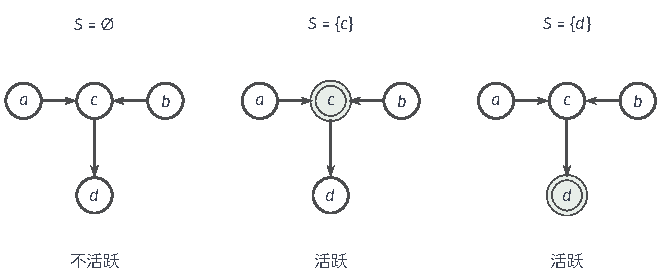
\includegraphics[width=112.0mm]{figures/01-mathematical-preliminaries-upper/05-graphs-and-signals/tikz/graph-theory-active-paths/figure.pdf}
  \caption{同一底层路径$a-c-b$在三个条件集下的活跃性。箭头及顶点没有改变；
  空条件集未打开碰撞点，给定碰撞点$c$或其后代$d$都会打开它。
  双圈表示被给定的顶点。活跃性不是沿箭头从$a$走到$b$的可达性，
  也不是简单删除条件顶点后的连通性。}
  \label{fig:graph-theory-active-paths}
\end{figure}

如图~\ref{fig:graph-theory-active-paths}所示，活跃性由箭头排列与$S$共同决定，
它既不是沿箭头的可达性，也不是删点后的无向连通性。
此外，一条路径被阻断不等于两端被分离，因为另一条路径可能仍活跃：
即使碰撞路径$a\to c\leftarrow b$在空条件下关闭，若同时存在链$a\to e\to b$，
$a,b$仍不分离。

\paragraph{分离规则的边界}
无向图里增大分隔集只会删除更多路径；DAG里加入碰撞点或其后代却可能重新打开路径，
两种变化方向相反，必须分开。更重要的是，d-分离目前只是图上的结构判据：
要把它解释成概率条件独立，还须联合分布按图分解这一额外假设，
而且结构上活跃也不保证某个具体分布里的相关系数一定非零。
概率与因果解释可参考\BookChapterRef{chap:causal-inference}{卷2《数学准备：概率、因果与决策》的“因果响应”章}。

\section{本章小结}

本章把四个层次的查询分清楚了。邻接检查一条边是否存在及其方向；
路径检查一条允许经过的顶点序列，并区分行走、简单路径与环，
再在给定边长意义下累计成本，注意负闭行走会使行走下确界变为$-\infty$；
连通把彼此可达的顶点归为分量，有向图还要区分强连通与弱连通，树则保证路径唯一；
条件分离检查的是给定$S$后全部底层路径是否活跃，规则随碰撞点及其后代而改变。

其中有三组判断尤其不能互换：最少边数与最低累计成本只在单位边长下一致；
弱连通与强连通在有向图里回答的是不同问题；
无向图“删点只会阻断”与DAG“给定碰撞点可能打开路径”方向相反。
下一章在此基础上讨论怎样实际检索：用队列和栈遍历、用排序确定执行次序、
用分量标记和生成森林组织顶点，用分块和树分解组织局部计算，
并把一次d-分离查询转换为无向可达查询。
